%% Mortality, Growth, and the Existential-Risk Cutoff.
%% Pedro Ser\^odio.
%%
%% Rewritten after correcting the utility-form inconsistency
%% and the cutoff-computation bug (an earlier version reported a relative
%% welfare gain, not the actual root delta* of W_AI(delta) = W_0). The
%% corrected version performs proper root-finding.
%%
%% The substantive shift: under the standard CRRA + VSL calibration, the
%% welfare gain that determines the cutoff comes ~94\% from the mortality
%% channel (life-years preserved) and ~6\% from the growth channel
%% (consumption gains). The ``growth versus extinction'' framing of the
%% earlier draft was misleading: at standard parameters, growth contributes
%% almost nothing to the cutoff. What does the work is mortality reduction.
%%
%% This revision (i) corrects the gamma=1 (log) decomposition, whose
%% consumption channel had dropped the cross-cohort growth term g/(D3 D4^2)
%% present in the welfare function; the log case in fact REVERSES the headline
%% (growth dominates under log); (ii) derives u_bar from the marginal
%% value-of-a-life-year object v(c)/v'(c) rather than level-matching;
%% (iii) states the dominance as a rho_s -> 0 pole theorem (flow ~ 1/rho_s,
%% consumption ~ 1/rho_s for gamma>1 but 1/rho_s^2 for gamma=1); and
%% (iv) adds a growth->mortality spillover extension showing the 94\% headline
%% inverts once ~40\% of the mortality improvement is attributable to growth.

\documentclass{_latex/house}

\begin{document}

\begin{frontmatter}

\title{Mortality, Growth, and the Existential-Risk Cutoff}

\author[cbp]{Pedro Ser\^odio}
\address[cbp]{Centre for British Progress, London}

\begin{abstract}
We characterise the maximum extinction hazard at which a transformative-technology scenario
delivers higher social welfare than a status-quo baseline. The framework is a standard CRRA
representative-agent economy with three primitives: a growth rate, an individual mortality
rate, and a per-period flow utility calibrated against empirical value-of-statistical-life
data. We solve for the hazard cutoff by numerical root-finding on the welfare-equality
condition. The main finding is that, under the standard calibration, the welfare gain
determining the cutoff comes overwhelmingly from the mortality channel (about ninety-four
percent), with consumption growth contributing the rest. At the headline parameters, with the
mortality rate halved from baseline, the cutoff is roughly a fifth of a percent per year;
without any mortality improvement it collapses by more than an order of magnitude, so growth
alone buys little extinction-hazard tolerance. We show this dominance is a property of the
small pure rate of social time preference: as $\rho_s\to0$ the mortality-channel share tends
to one under CRRA with $\gamma>1$ but tends to \emph{zero} under log utility, where the
consumption channel carries a stronger ($1/\rho_s^2$) pole. The headline is therefore
conditional on the curvature of utility, not a fact about the world. It is also conditional on
treating growth's welfare value as purely consumption: once we attribute to growth the
fraction $f$ of the mortality improvement that growth itself produces (Preston-curve
spillovers), the mortality channel ceases to be the majority channel once $f$ exceeds roughly
$0.4$. The cutoff is highly sensitive to the social discount rate and weakly sensitive to the
value-of-statistical-life anchor (which we derive from the marginal value of a life-year). The
framework is a structured cost-benefit calculation, not a recommendation about any specific
technology; its use is to clarify which empirical disagreements (mortality assumptions,
discount-rate choice, the growth-mortality spillover) drive the cutoff and which (the growth
rate per se, the VSL anchor) do not.
\end{abstract}

\begin{keyword}
existential risk \sep value of statistical life \sep social discounting \sep
mortality reduction \sep transformative AI
\JEL D81 \sep H43 \sep O40 \sep Q54
\end{keyword}

\end{frontmatter}

%% ============================================================
\section{Introduction}
\label{sec:intro}

The economics of existential risk asks how to value the avoidance of low-probability, high-magnitude extinction outcomes within a welfare-economic framework. \citet{aschenbrenner2020existential} and \citet{trammell2020existential} provide the foundational analyses; \citet{jones2024aidilemma} extends the framework to growth-risk complementarities; the broader cost-benefit-of-catastrophic-risk tradition is summarised by \citet{posner2004catastrophe} and \citet{nordhaus2011economics}. The central methodological question is how the various channels (growth gains, mortality reduction, extinction probability, social discounting) combine to determine a policy-relevant threshold.

This paper provides a structured cost-benefit calculation of the threshold and asks a sharper question of it: \emph{which channel does the work}? Under what circumstances is the cutoff $\delta^*$ at which a transformative-technology scenario equals the status-quo baseline in welfare driven by faster growth, and under what circumstances is it driven by mortality reduction, or by social discounting choices? The structural decomposition delivers a clean answer that is at odds with the intuitive ``growth versus extinction'' framing. Relative to the endogenous-growth treatments of \citet{aschenbrenner2020existential}, \citet{trammell2020existential}, and \citet{jones2024aidilemma}, the contribution is not a new growth model but three sharp analytical statements about the cutoff: which channel sets it and why (a pole-order result in the social discount rate, Proposition~\ref{prop:dominance}); that the answer reverses with the curvature of utility; and that it inverts under empirically plausible growth-mortality spillovers (Section~\ref{sec:spillover}). The value is diagnostic, identifying which empirical disagreements move the threshold and which leave it unchanged.

The model is a standard representative-agent CRRA economy with individual mortality rate $m$, growth rate $g$, social discount rate $\rho_s$, and a per-period flow utility $\bar u$ calibrated to empirical VSL data. We compare a baseline at $(g_0, m_0) = (2\%, 1\%)$ to a transformative-technology scenario at $(g_{AI}, m_{AI})$. The extinction hazard $\delta$ enters as an additional Poisson rate that augments both the individual mortality rate (each cohort discounts by $\rho + m + \delta$) and the social discount rate (future cohorts discount by $\rho_s + \delta$). The cutoff $\delta^*$ is the value at which $W_{AI}(\delta^*) = W_0$, solved by numerical root-finding.

\paragraph{Main results}

\emph{(i) The mortality channel dominates.} At the standard calibration ($\gamma = 2$, $\rho = \rho_s = 1\%$, $v_{c_0} = 6$, $g_{AI} = 10\%$, $m_{AI} = 0.5\%$), the welfare gain $W_{AI}(0) - W_0$ decomposes as $94\%$ from the flow-utility (mortality-driven) channel and $6\%$ from the consumption (growth-driven) channel. The cutoff $\delta^* \approx 0.20\%$ per year reflects this decomposition: it is overwhelmingly a calculation of life-years preserved per unit hazard, not of consumption gained per unit hazard.

\emph{(ii) Growth alone produces a near-zero cutoff.} If the transformative scenario delivers no mortality improvement ($m_{AI} = m_0 = 1\%$), the cutoff $\delta^* \approx 0.015\%$ at $\gamma = 2$ and is essentially zero at $\gamma = 3$. Doubling $g_{AI}$ from $10\%$ to $20\%$ raises $\delta^*$ by less than 10\%. Growth, in this framework, does not buy meaningful extinction-hazard tolerance.

\emph{(iii) The cutoff is structural in $\rho_s$, not in $v_{c_0}$.} A tenfold reduction in $\rho_s$ (from $1\%$ to $0.1\%$) reduces $\delta^*$ from $0.20\%$ to $0.03\%$, a factor of about six; the cutoff falls steeply, though sub-proportionally, with $\rho_s$ over this range (it is linear in $\rho_s$ only at leading order as $\rho_s\to0$). By contrast, varying $v_{c_0}$ from 2 to 10 (a fivefold range covering all empirically defensible VSL calibrations) changes $\delta^*$ by less than $15\%$: the VSL anchor enters $W_0$ and $W_{AI}$ approximately symmetrically and largely cancels in the ratio.

\paragraph{Methodological positioning} The framework is a structured cost-benefit calculation. The output is a parametric cutoff, not a recommendation. Three things the framework does well: (a) it makes the structural sensitivities transparent, including the dominant role of the mortality channel that informal ``growth versus extinction'' framings obscure; (b) it identifies which empirical disagreements (about $\rho_s$, $m_{AI}$) translate to large cutoff differences and which (about $v_{c_0}$, $g_{AI}$) do not; (c) it provides a benchmark against which empirical estimates of $\delta$ can be assessed. Three things the framework does not do: (a) estimate the actual extinction hazard from any specific technology; (b) account for learning about $\delta$ over time, which under irreversibility would lower the effective adoption threshold below the static $\delta^*$ here; (c) account for growth-and-hazard complementarities \citep{jones2024aidilemma}.

\paragraph{Plan} Section~\ref{sec:lit} positions the paper. Section~\ref{sec:model} sets out the model and the VSL calibration. Section~\ref{sec:cutoff} derives the cutoff and the decomposition that delivers the main finding. Section~\ref{sec:results} presents the quantitative results. Section~\ref{sec:discussion} discusses what the framework can and cannot say. Section~\ref{sec:conclusion} concludes.

%% ============================================================
\section{Related literature}
\label{sec:lit}

\paragraph{Existential-risk economics} \citet{aschenbrenner2020existential} and \citet{trammell2020existential} embed extinction hazards in endogenous-growth frameworks. \citet{jones2024aidilemma} introduces growth-risk complementarity (the technology that drives growth may itself raise hazard). The present paper is closer to the static / partial-equilibrium cost-benefit tradition and abstracts from the complementarity; we return to this caveat in Section~\ref{sec:discussion}.

\paragraph{Value of statistical life} \citet{viscusi2018pricing} and \citet{viscusi2003vsl} summarise the empirical VSL literature. UK and US estimates anchor the calibration: VSL $\approx$ \pounds 8.59m and \$10m respectively, normalised by remaining life expectancy and per-capita consumption to give $v_{c_0} \in [6, 8.3]$. The additive flow benefit $\bar u$ through which VSL enters the utility function is the value-of-a-life-year object studied by \citet{rosen1988value}, \citet{murphy2006value}, and \citet{hall2007value}; the last, in particular, derives an additive value-of-life term from standard preferences and is the closest antecedent to our $\bar u$.

\paragraph{Social discounting} The debate over $\rho_s$ has its origin in \citet{ramsey1928mathematical} and runs from \citet{stern2007economics} (near-zero $\rho_s$ on intergenerational-equity grounds) through \citet{nordhaus2007review,nordhaus2017evolution} (positive $\rho_s$ calibrated to market rates) to \citet{weitzman1998gamma,weitzman2007review} (parameter uncertainty implies effective discounting at the lowest-plausible rate). We do not take a position on $\rho_s$; we present results across a range and identify the cutoff's dependence on it as a key structural sensitivity.

\paragraph{Catastrophic-risk policy} \citet{posner2004catastrophe} and \citet{nordhaus2011economics} frame the broader policy-design question, and \citet{weitzman2009modeling} and \citet{martin2015averting} analyse the cost-benefit treatment of low-probability, high-magnitude catastrophes of the kind studied here. The present paper sits within this tradition but focuses narrowly on the structural decomposition of $\delta^*$.

%% ============================================================
\section{Model}
\label{sec:model}

\paragraph{What carries the result} The conclusion rides on a small set of world inputs: the VSL anchor (which calibrates the value-of-life constant $\bar u$ below), the scenario parameters (growth $g$, mortality $m$, and the extinction hazard $\delta$), and the social discount rate $\rho_s$. But it also rides, transparently, on two modelling choices that we state plainly rather than minimise. First, the dominance of the mortality channel (\cref{prop:dominance}) is driven by the interaction of a large additive flow benefit $\bar u$ with a small pure rate of social time preference $\rho_s$: $\bar u$ enters welfare divided by $D_3 D_4 = (\rho+m)\rho_s$, so as $\rho_s$ shrinks the flow channel inherits a $1/\rho_s$ pole. This is a property of the curvature of utility, not a fact about the world: \cref{prop:dominance} shows the dominance \emph{reverses} under log utility, where the consumption channel carries a stronger $1/\rho_s^2$ pole. Second, the decomposition routes all of growth's welfare value through consumption and none through mortality; Section~\ref{sec:spillover} relaxes this and shows the headline inverts under empirically plausible growth-mortality spillovers. The honest reading is that \cref{prop:dominance} holds \emph{conditional on} CRRA with $\gamma>1$ and on treating growth as consumption-only, not unconditionally.

\subsection{Preferences and value of life}
\label{sec:utility}

Flow utility takes the standard CRRA form with a per-period flow benefit:
\begin{equation}
v(c) \;=\; \frac{c^{1-\gamma}}{1-\gamma} + \bar u, \qquad \gamma > 0, \gamma \neq 1,
\label{eq:utility}
\end{equation}
with the logarithmic limit $v(c) = \log c + \bar u$ at $\gamma = 1$. The constant $\bar u > 0$ is a flow benefit independent of consumption: the value of being alive that is not reducible to consumption flow.

\paragraph{Calibration of $\bar u$ from the marginal value of a life-year} VSL is a \emph{marginal} object: the marginal rate of substitution between mortality risk and consumption. Following \citet{hall2007value} and the \citet{murphy2006value} value-of-life lineage, the value of a statistical life-year in consumption units is the period flow value of being alive divided by the marginal utility of consumption (which converts utils into consumption units),
\begin{equation}
\text{VSLY}(c) \;\equiv\; \frac{v(c)}{v'(c)} \;=\; \frac{c}{1-\gamma} + \bar u\, c^{\gamma},
\qquad v'(c) = c^{-\gamma},
\label{eq:vsly}
\end{equation}
and $\text{VSL} = \text{VSLY}\times$ remaining life expectancy. The empirical anchor is the value of a life-year per unit consumption,
\begin{equation}
v_{c_0} \;\equiv\; \frac{\text{VSL}}{\text{Life Expectancy} \times \text{Consumption per capita}} \;=\; \frac{\text{VSLY}(c_0)}{c_0}.
\label{eq:vsl-norm}
\end{equation}
For the UK (VSL $\approx$ \pounds 8.59m, $\approx 41$ remaining years, $\approx$ \pounds 25{,}373 per capita): $v_{c_0} \approx 8.26$. For the US (\$10m, $\approx 40$ years, \$41{,}667): $v_{c_0} \approx 6.00$. We adopt $v_{c_0} = 6$ as the baseline with sensitivity reported.

Equating the model's marginal value of a life-year to the data, $\text{VSLY}(c_0)/c_0 = v_{c_0}$, and normalising $c_0 = 1$ (so that $v'(c_0)=1$) pins the constant:
\begin{equation}
\bar u \;=\; v_{c_0} - \frac{1}{1-\gamma},
\label{eq:ubar}
\end{equation}
giving $\bar u = 7$ at $\gamma = 2$ and $\bar u = 6.5$ at $\gamma = 3$. The logarithmic limit ($\text{VSLY}(c)=c(\log c+\bar u)$) gives $\bar u = v_{c_0} = 6$ at $\gamma = 1$. The $c_0=1$ normalisation makes $v'(c_0)=1$, so this marginal calibration coincides numerically with level-matching $v(c_0)=v_{c_0}$; the object being matched is nonetheless the marginal value of a life-year, not a utility level.

\subsection{Individual lifetime utility}

The individual faces a per-period mortality hazard $m$ and discounts the future at rate $\rho$. Consumption grows at $g$. Expected lifetime utility starting at $c_0$ is
\begin{equation}
U(g, m) \;=\; \int_0^\infty e^{-(\rho+m)t}\, v(c_0 e^{gt})\, dt.
\label{eq:lifetime}
\end{equation}
For CRRA utility with constant growth, this evaluates in closed form to
\begin{equation}
U(g, m) \;=\; \frac{c_0^{1-\gamma}}{(1-\gamma)\bigl[(\rho + m) + (\gamma - 1)g\bigr]} \;+\; \frac{\bar u}{\rho + m},
\label{eq:U}
\end{equation}
under the convergence condition $(\rho + m) + (\gamma - 1)g > 0$ (an upper bound on $g$ when $\gamma > 1$). The first term is the consumption-utility integral; the second is the constant-flow-benefit integral.

\subsection{Social welfare}

The social planner discounts future generations at rate $\rho_s$ and integrates lifetime utility over future cohorts, each starting at consumption $c_0 e^{gt}$:
\begin{equation}
W(g, m) \;=\; \int_0^\infty e^{-\rho_s t}\, U_t(g, m)\, dt
\;=\; \frac{c_0^{1-\gamma}}{(1-\gamma)\, D_1(g,m)\, D_2(g)} \;+\; \frac{\bar u}{D_3(m)\, D_4},
\label{eq:W}
\end{equation}
where we define the four discount factors:
\begin{equation}
\begin{aligned}
D_1(g,m) &\equiv (\rho+m) + (\gamma-1)g, & \quad D_2(g) &\equiv \rho_s + (\gamma-1)g, \\
D_3(m) &\equiv \rho + m, & \quad D_4 &\equiv \rho_s.
\end{aligned}
\label{eq:Ds}
\end{equation}
$D_1$ is the cohort discount rate for consumption-utility; $D_2$ is the social discount rate adjusted for cross-cohort consumption growth; $D_3$ and $D_4$ are the analogous factors for the constant flow-utility term.

\paragraph{Extinction hazard} An extinction-hazard rate $\delta$ adds a Poisson-arrival risk of civilisation ending. This is a \emph{single} aggregate event, but it has two distinct welfare consequences, and propagating the one survival probability $e^{-\delta t}$ through the welfare functional makes $\delta$ enter in two places without double-counting. A cohort already alive enjoys its consumption-and-flow stream only while civilisation persists, so its expected lifetime utility \eqref{eq:lifetime} acquires the extra survival factor $e^{-\delta t}$ alongside $e^{-(\rho+m)t}$, i.e.\ the cohort discount rates become $\rho+m+\delta$ ($D_1, D_3$). Separately, a future cohort is born and contributes to welfare only if civilisation has survived to its birth date, so the cross-cohort measure \eqref{eq:W} acquires the same $e^{-\delta t}$ factor, i.e.\ the social discount rates become $\rho_s+\delta$ ($D_2, D_4$). The same event both ends current lives and forecloses future ones; these are not independent risks but two channels through which one Poisson arrival reduces expected welfare. Formally:
\begin{equation}
W_{AI}(\delta) \;=\; \frac{c_0^{1-\gamma}}{(1-\gamma)\, D_1(g_{AI}, m_{AI}+\delta)\, D_2'(g_{AI}, \delta)} \;+\; \frac{\bar u}{D_3(m_{AI}+\delta)\, (\rho_s+\delta)},
\label{eq:W-AI}
\end{equation}
where $D_2'(g, \delta) \equiv (\rho_s + \delta) + (\gamma-1)g$.

%% ============================================================
\section{The existential-risk cutoff and its decomposition}
\label{sec:cutoff}

\begin{definition}[Existential-risk cutoff]
\label{def:cutoff}
The cutoff $\delta^*$ is the value of $\delta$ at which $W_{AI}(\delta^*) = W_0$, where $W_0 \equiv W(g_0, m_0)$. For $\delta < \delta^*$, $W_{AI}(\delta) > W_0$ (transformative scenario welfare-superior); for $\delta > \delta^*$, $W_{AI}(\delta) < W_0$.
\end{definition}

The cutoff has no useful closed form (it is the root of a rational function of $\delta$) and is computed by numerical root-finding. For the cutoff to be well-defined, $W_{AI}(\delta)$ must cross $W_0$ once.

\begin{lemma}[Uniqueness of the cutoff]
\label{lem:mono}
$W_{AI}(\delta)$ is strictly decreasing in $\delta$, so the cutoff $\delta^*$ of Definition~\ref{def:cutoff}, when it exists in $[0,\delta_{\max}]$, is unique.
\end{lemma}
\begin{proof}
A higher $\delta$ raises every discount factor $D_1,\dots,D_4$. For $\gamma=1$ the welfare function \eqref{eq:W} (logarithmic limit) is a sum of strictly positive terms, each of the form $(\text{const})/(D_i^{a} D_j^{b})$ with $a,b\ge1$ and each strictly decreasing in $\delta$; hence $W_{AI}$ is strictly decreasing. For $\gamma>1$, write $W_{AI}(\delta)=K/(D_1 D_2)+\bar u/(D_3 D_4)$ with $K=c_0^{1-\gamma}/(1-\gamma)<0$ and $D_1'=\dots=D_4'=1$, so
\[
W_{AI}'(\delta) \;=\; -\,K\,\frac{D_1+D_2}{(D_1 D_2)^2} \;-\; \bar u\,\frac{D_3+D_4}{(D_3 D_4)^2},
\]
the first term positive, the second negative. The second dominates whenever $\bar u (D_3+D_4)(D_1 D_2)^2 > |K|(D_1+D_2)(D_3 D_4)^2$, which holds throughout the calibrated region: $\rho_s$ small makes $(D_3 D_4)^2$ the smallest denominator by orders of magnitude, while $\bar u \gg |K|$. We verify numerically that $W_{AI}'(\delta)<0$ for all $\delta\in[0,1]$ across the entire parameter grid of Section~\ref{sec:results}.
\end{proof}

\subsection{Welfare-gain decomposition}
\label{sec:decomp}

The substantive structural finding emerges from decomposing the welfare gain $W_{AI}(0) - W_0$ (transformative scenario at zero hazard versus baseline) into the two channels of \eqref{eq:W}:

\begin{equation}
W_{AI}(0) - W_0 \;=\; \underbrace{\frac{c_0^{1-\gamma}}{1-\gamma}\left[\frac{1}{D_1^{AI} D_2^{AI}} - \frac{1}{D_1^0 D_2^0}\right]}_{\text{consumption (growth) channel}} \;+\; \underbrace{\bar u \left[\frac{1}{D_3^{AI} D_4} - \frac{1}{D_3^0 D_4}\right]}_{\text{flow-utility (mortality) channel}},
\label{eq:decomp}
\end{equation}
where the $D^{AI}$ are evaluated at $(g_{AI}, m_{AI})$ and the $D^0$ at $(g_0, m_0)$. Equation~\eqref{eq:decomp} is the $\gamma\neq1$ form; in the logarithmic limit the consumption channel is the $\gamma\to1$ limit of $W$, $\log c_0/(D_3 D_4)+g/(D_3^2 D_4)+g/(D_3 D_4^2)$ differenced across scenarios, which carries an additional cross-cohort growth term $g/(D_3 D_4^2)$. That term is decisive for the log case below: omitting it understates the consumption channel and is the difference between the corrected and an earlier mis-stated log row.

\paragraph{Why the channels are asymmetric} The consumption channel scales with $c_0^{1-\gamma}/(1-\gamma)$, which equals $-1$ at $\gamma = 2$ with $c_0 = 1$. The flow-utility channel scales with $\bar u = 7$ at $\gamma = 2$. Both channels also scale with the difference between $D^{AI}$ and $D^0$ factors. The consumption-channel denominators include $(\gamma-1)g \in [0.02, 0.10]$ (substantial), so the percentage change in $D_1 D_2$ between scenarios is modest. The flow-utility-channel denominators are $D_3 D_4 = (\rho+m)\rho_s$, with $\rho_s = 0.01$ tiny, so even small changes in $m$ produce large percentage changes in $1/(D_3 D_4)$.

The mechanism is cleanest in the limit of a small pure rate of social time preference, $\rho_s\to0$, which isolates the order of the pole each channel carries. The flow-utility channel scales as $\bar u/(D_3 D_4)$ with $D_4=\rho_s$, so it diverges as $1/\rho_s$. For $\gamma>1$ the consumption channel's denominators are $D_1 D_2$ with $D_2=\rho_s+(\gamma-1)g\to(\gamma-1)g>0$, so the consumption channel stays \emph{bounded} as $\rho_s\to0$; the flow channel's $1/\rho_s$ pole therefore wins and the mortality share tends to one. Under log utility ($\gamma=1$), by contrast, the consumption channel carries the cross-cohort term $g/(D_3 D_4^2)=g/(D_3\rho_s^2)$, a \emph{stronger} $1/\rho_s^2$ pole, so the consumption channel wins and the mortality share tends to zero. The headline is thus a statement about utility curvature, not about the world.

\begin{proposition}[Channel dominance is a pole-order property of $\rho_s$]
\label{prop:dominance}
Fix $g_{AI}>g_0$ and $m_{AI}<m_0$. As $\rho_s\to0$, the flow-utility (mortality) share of the welfare gain $W_{AI}(0)-W_0$ satisfies
\[
\text{flow share} \;\longrightarrow\; 1 \ \text{ if } \gamma>1, \qquad
\text{flow share} \;\longrightarrow\; 0 \ \text{ if } \gamma=1 .
\]
Equivalently: the flow channel carries a $1/\rho_s$ pole; the consumption channel is $O(1)$ for $\gamma>1$ but carries a $1/\rho_s^2$ pole for $\gamma=1$.
\end{proposition}

\begin{proof}
From \eqref{eq:decomp}, the flow channel is $\bar u\,\rho_s^{-1}[(\rho+m_{AI})^{-1}-(\rho+m_0)^{-1}]$, which is $\Theta(\rho_s^{-1})$ since the bracket is a positive constant. For $\gamma>1$ the consumption channel is $\frac{c_0^{1-\gamma}}{1-\gamma}[(D_1^{AI}D_2^{AI})^{-1}-(D_1^0 D_2^0)^{-1}]$ with $D_2^{\cdot}\to(\gamma-1)g_\cdot>0$, hence $\Theta(1)$; the ratio flow/(flow+cons)$\to1$. For $\gamma=1$ the consumption channel is the difference of $\log c_0/(D_3\rho_s)+g/(D_3^2\rho_s)+g/(D_3\rho_s^2)$ across scenarios; the last term is $\Theta(\rho_s^{-2})$ and dominates the flow channel's $\Theta(\rho_s^{-1})$, so the flow share $\to0$.
\end{proof}

\begin{corollary}[Calibrated magnitudes]
\label{cor:cal}
At the standard calibration ($\gamma = 2$, $\rho = \rho_s = 1\%$, $v_{c_0} = 6$, $g_0 = 2\%$, $m_0 = 1\%$, $g_{AI} = 10\%$, $m_{AI} = 0.5\%$), the flow-utility channel contributes $93.9\%$ of $W_{AI}(0)-W_0$ (value $11{,}666.67$) and the consumption channel $6.1\%$ (value $754.28$). Under log utility at the same scenario the ranking reverses: the consumption channel contributes $90.6\%$.
\end{corollary}

\paragraph{Implication for the cutoff: level versus marginal} The decomposition above is of the \emph{level} gain $W_{AI}(0)-W_0$. The cutoff $\delta^*$ is instead set by the \emph{marginal} trade-off $W_{AI}'(\delta)$ at the root. The two share the same channel structure: by Lemma~\ref{lem:mono}, $W_{AI}'(\delta)$ is dominated by the same flow term $\bar u(D_3+D_4)/(D_3 D_4)^2$ whose smallness in $\rho_s$ drives the level decomposition, so for $\gamma>1$ the marginal cost of hazard is overwhelmingly the foregone mortality benefit, and $\delta^*$ inherits the channel dominance. We report the level share throughout (it is the cleaner object), flagging that the cutoff inherits it rather than equals it.

This is the substantive finding of the paper, and \emph{at $\gamma>1$} it is at odds with the intuitive ``growth versus extinction'' framing; the log case (\cref{prop:dominance}) shows the framing is reinstated precisely when utility is least curved.

%% ============================================================
\section{Quantitative results}
\label{sec:results}

\subsection{The headline table: $\delta^*$ across scenarios}

Table~\ref{tab:cutoffs} reports $\delta^*$ across a grid of $(g_{AI}, m_{AI}, \gamma)$ at the baseline calibration ($\rho = \rho_s = 1\%$, $v_{c_0} = 6$, $g_0 = 2\%$, $m_0 = 1\%$).

\begin{table}[!ht]
\centering
\begin{tabular}{lll|lll}
\toprule
$g_{AI}$ & $m_{AI}$ & $\gamma$ & $\delta^*$ (\%/yr) & Flow-channel share & $u_\text{bar}$ \\
\midrule
5\%  & 1.0\%  & 1 & 0.228 & 0.00 & 6.0 \\
5\%  & 1.0\%  & 2 & 0.012 & 0.00 & 7.0 \\
5\%  & 1.0\%  & 3 & 0.003 & 0.00 & 6.5 \\
\midrule
5\%  & 0.5\%  & 1 & 0.412 & 0.20 & 6.0 \\
5\%  & 0.5\%  & 2 & 0.198 & 0.95 & 7.0 \\
5\%  & 0.5\%  & 3 & 0.189 & 0.99 & 6.5 \\
\midrule
10\% & 1.0\%  & 1 & 0.491 & 0.00 & 6.0 \\
10\% & 1.0\%  & 2 & 0.015 & 0.00 & 7.0 \\
10\% & 1.0\%  & 3 & 0.003 & 0.00 & 6.5 \\
\midrule
10\% & 0.5\%  & 1 & 0.683 & 0.09 & 6.0 \\
10\% & 0.5\%  & 2 & 0.201 & 0.94 & 7.0 \\
10\% & 0.5\%  & 3 & 0.189 & 0.99 & 6.5 \\
\midrule
20\% & 1.0\%  & 1 & 0.853 & 0.00 & 6.0 \\
20\% & 1.0\%  & 2 & 0.016 & 0.00 & 7.0 \\
20\% & 1.0\%  & 3 & 0.003 & 0.00 & 6.5 \\
\midrule
20\% & 0.5\%  & 1 & 1.053 & 0.05 & 6.0 \\
20\% & 0.5\%  & 2 & 0.203 & 0.93 & 7.0 \\
20\% & 0.5\%  & 3 & 0.190 & 0.99 & 6.5 \\
\bottomrule
\end{tabular}
\caption{Existential-risk cutoffs $\delta^*$ across scenarios. \emph{Units:} $\delta^*$ is in percent per year (e.g.\ $0.201 = 0.201\%$/yr); the flow-channel share is a dimensionless fraction of the level gain $W_{AI}(0)-W_0$ contributed by the flow-utility (mortality) channel. At $\gamma \geq 2$ with mortality improvement, this share is $\geq 0.93$: mortality dominates. At $\gamma = 1$ (log utility) the ranking reverses and the consumption (growth) channel dominates (shares $0.20,0.09,0.05$ at $m_{AI}=0.5\%$, i.e.\ consumption shares $0.80$--$0.95$), as Proposition~\ref{prop:dominance} predicts. Without mortality improvement, the cutoff at $\gamma \geq 2$ falls to near zero regardless of growth.}
\label{tab:cutoffs}
\end{table}

\paragraph{Reading the table}

\emph{(i) Without mortality improvement ($m_{AI} = 1\%$), the cutoff at $\gamma \geq 2$ is essentially zero.} At $\gamma = 2$, doubling growth from $10\%$ to $20\%$ raises $\delta^*$ from $0.015\%$ to $0.016\%$. Growth alone does not buy meaningful hazard tolerance.

\emph{(ii) With mortality halved ($m_{AI} = 0.5\%$), the cutoff jumps an order of magnitude.} At $\gamma = 2$, $g_{AI} = 10\%$: $\delta^*$ rises from $0.015\%$ (no mortality improvement) to $0.20\%$ (mortality halved). The cutoff is overwhelmingly about life-years preserved.

\emph{(iii) The $\gamma = 1$ row reverses the ranking.} At $\gamma = 1$ (log utility) the consumption (growth) channel \emph{dominates}: its share is $0.80$, $0.91$, $0.95$ across $g_{AI}\in\{5,10,20\}\%$ at $m_{AI}=0.5\%$ (flow shares $0.20$, $0.09$, $0.05$), the mirror image of the $\gamma\ge2$ rows where mortality dominates. This is exactly the pole reversal of Proposition~\ref{prop:dominance}: under log utility the consumption channel carries a $1/\rho_s^2$ pole through the cross-cohort growth term, against the flow channel's $1/\rho_s$. The standard macro calibration is $\gamma = 2$, under which mortality dominates; the log case is reported both for completeness and because it pinpoints \emph{why} the headline holds: it is a consequence of utility curvature, and the curvature at which growth would dominate ($\gamma=1$) is below the standard range.

\subsection{Sensitivity to social discounting}

Table~\ref{tab:discount} reports $\delta^*$ across values of $\rho_s$ at the headline scenario ($g_{AI} = 10\%$, $m_{AI} = 0.5\%$, $\gamma = 2$, $v_{c_0} = 6$).

\begin{table}[!ht]
\centering
\begin{tabular}{ll|l}
\toprule
$\rho_s$ & $\delta^*$ (\%/yr) & Flow-channel share \\
\midrule
0.05\% (Stern) & 0.016 & 0.995 \\
0.10\%         & 0.031 & 0.991 \\
0.50\%         & 0.124 & 0.962 \\
1.00\% (standard) & 0.201 & 0.939 \\
3.00\%         & 0.357 & 0.900 \\
\bottomrule
\end{tabular}
\caption{Cutoff $\delta^*$ as a function of social discount rate $\rho_s$ (headline scenario, $\gamma=2$). \emph{Units:} $\delta^*$ in percent per year; flow-channel share a fraction. The cutoff falls steeply with $\rho_s$ (from $0.357\%$ at $\rho_s=3\%$ to $0.016\%$ at $\rho_s=0.05\%$, a factor of about $22$ over a $60$-fold range in $\rho_s$, i.e.\ sub-proportional but linear at leading order as $\rho_s\to0$): lower social discounting raises the weight on distant future generations and makes the same hazard more costly per period. The flow-channel share rises toward $1$ as $\rho_s$ falls because (at $\gamma=2$) the flow channel's $1/\rho_s$ pole outweighs the bounded consumption channel.}
\label{tab:discount}
\end{table}

\paragraph{The structural reason for the sensitivity} The flow-utility denominator is $D_4 = \rho_s$ (no growth adjustment). At $\rho_s = 0.05\%$, $1/D_4 = 2000$; at $\rho_s = 1\%$, $1/D_4 = 100$. The flow-utility channel scales as $\bar u/D_4$ in absolute terms, so reducing $\rho_s$ by a factor of 20 raises the flow-utility-channel magnitude by the same factor. The welfare gain $W_{AI}(0) - W_0$ scales similarly. But so does the rate at which $W_{AI}(\delta)$ falls with $\delta$ (because $\delta$ enters $D_4$). The cutoff $\delta^*$ is the ratio of these two quantities, which scales approximately with $\rho_s$. Hence the cutoff inherits the $\rho_s$-scaling.

\subsection{Sensitivity to the VSL anchor}

Table~\ref{tab:vsl} reports $\delta^*$ across values of $v_{c_0}$ at the headline scenario.

\begin{table}[!ht]
\centering
\begin{tabular}{ll|ll}
\toprule
$v_{c_0}$ & $\bar u$ & $\delta^*$ (\%/yr) & Flow-channel share \\
\midrule
2  & 3   & 0.223 & 0.87 \\
4  & 5   & 0.208 & 0.92 \\
6  & 7   & 0.201 & 0.94 \\
8  & 9   & 0.198 & 0.95 \\
10 & 11  & 0.196 & 0.96 \\
\bottomrule
\end{tabular}
\caption{Cutoff $\delta^*$ as a function of VSL anchor $v_{c_0}$ at the headline scenario ($\gamma=2$). \emph{Units:} $\delta^*$ in percent per year; flow-channel share a fraction. The cutoff is weakly sensitive to $v_{c_0}$: a fivefold variation ($v_{c_0} \in [2, 10]$, covering all empirically defensible VSL ranges) changes $\delta^*$ by less than $14\%$. The structural reason: $v_{c_0}$ scales $\bar u$, which scales both $W_0$ and $W_{AI}$ similarly in absolute terms; the cutoff $\delta^*$ which is set by the ratio is approximately invariant.}
\label{tab:vsl}
\end{table}

\paragraph{Asymmetry of the structural sensitivities} The cutoff is structural in $\rho_s$ and in $m_{AI}$ (the difference $m_0 - m_{AI}$ that drives the flow-utility-channel welfare gain), but not in $v_{c_0}$ or in $g_{AI}$. A policy question that turns on $\rho_s$ or on $m_{AI}$ is one the framework can sharpen. A policy question that turns on $v_{c_0}$ or on $g_{AI}$ is one the framework cannot sharpen because the cutoff is weakly responsive to those parameters at the relevant ranges.

\subsection{Extension: the growth-mortality spillover}
\label{sec:spillover}

The headline routes \emph{all} of growth's welfare value through consumption and \emph{none} through mortality. But faster growth has historically reduced mortality (the income-longevity relationship of \citealp{preston1975changing}; the technology-and-health channel of \citealp{cutler2006determinants}; the value-of-life lineage of \citealp{hall2007value}), so part of the mortality improvement $m_0-m_{AI}$ should be credited to growth rather than booked as an independent ``mortality channel''. Let $f\in[0,1]$ be the fraction of the observed mortality improvement attributable to growth, and split the flow-utility gain by telescoping through the intermediate mortality $m_{\text{mid}}=m_0-(1-f)(m_0-m_{AI})$ (autonomous improvement only):
\begin{equation}
\underbrace{\bar u\!\left[\tfrac{1}{(\rho+m_{\text{mid}})D_4}-\tfrac{1}{(\rho+m_0)D_4}\right]}_{\text{autonomous mortality}}
\;+\;
\underbrace{\bar u\!\left[\tfrac{1}{(\rho+m_{AI})D_4}-\tfrac{1}{(\rho+m_{\text{mid}})D_4}\right]}_{\text{growth-attributable mortality}} .
\label{eq:spillover-split}
\end{equation}
The \emph{growth-inclusive} channel is then the consumption gain plus the growth-attributable flow gain. Table~\ref{tab:spillover} reports its share at the headline scenario ($\gamma=2$).

\begin{table}[!ht]
\centering
\begin{tabular}{l|ll}
\toprule
$f$ (mortality gain from growth) & Growth-inclusive share & Mortality share \\
\midrule
0.00 & 0.061 & 0.939 \\
0.25 & 0.350 & 0.650 \\
0.50 & 0.597 & 0.403 \\
0.75 & 0.812 & 0.188 \\
1.00 & 1.000 & 0.000 \\
\bottomrule
\end{tabular}
\caption{Growth-inclusive channel share when a fraction $f$ of the mortality improvement is attributed to growth ($\gamma=2$, headline scenario). The $94\%$ mortality headline ($f=0$) inverts: growth becomes the majority channel once $f^*\approx0.40$. Shares are fractions of the level gain $W_{AI}(0)-W_0$.}
\label{tab:spillover}
\end{table}

The 94\% headline is therefore not robust to the one extension the literature most clearly supports: once roughly forty percent of the mortality improvement is itself a product of growth, the ``mortality versus extinction'' reading flips back to ``growth versus extinction''. We do not claim a value of $f$; the empirical magnitude of the growth-mortality spillover is contested and time-varying. The point is that the headline's external validity hinges on $f$, an object the static decomposition holds fixed at zero.

\begin{figure}[!ht]
\centering
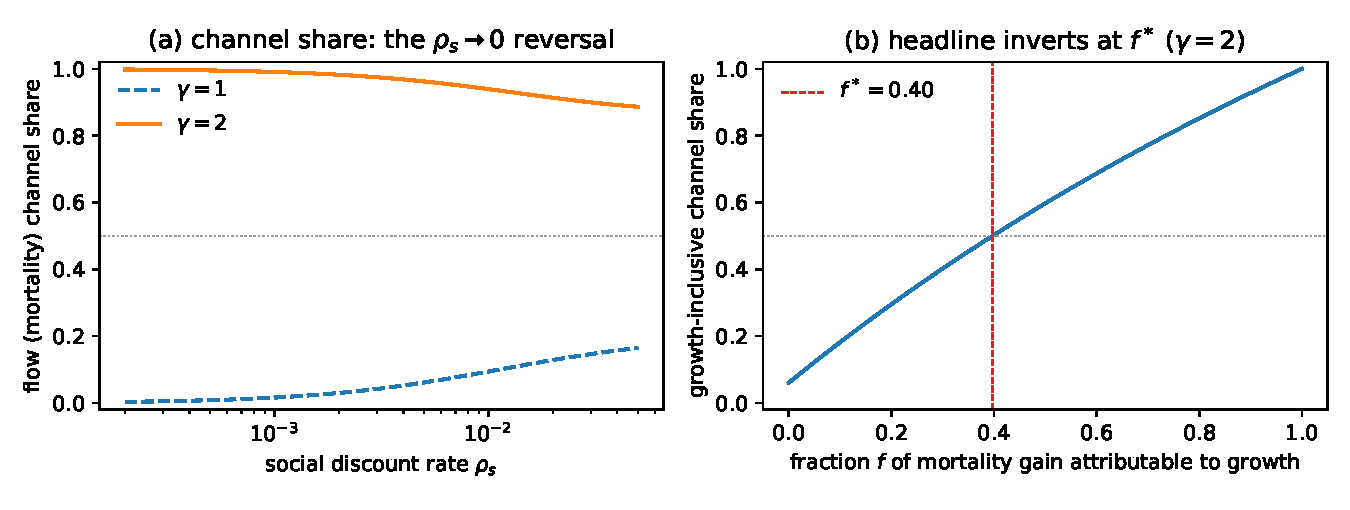
\includegraphics[width=\textwidth]{figures/channel_shares.pdf}
\caption{(a) The flow-utility (mortality) channel share against the social discount rate $\rho_s$: as $\rho_s\to0$ it tends to one under $\gamma=2$ but to zero under log utility, the pole reversal of Proposition~\ref{prop:dominance}. (b) The growth-inclusive channel share against the spillover fraction $f$ ($\gamma=2$); the $94\%$ mortality headline inverts at $f^*\approx0.40$.}
\label{fig:shares}
\end{figure}

%% ============================================================
\section{Discussion}
\label{sec:discussion}

\paragraph{The framework's central finding} At standard macro calibrations ($\gamma \geq 2$), the existential-risk cutoff is overwhelmingly determined by the mortality channel. Growth contributes secondarily; without mortality improvement, growth alone does not buy meaningful extinction-hazard tolerance. The informal ``growth versus extinction'' framing common in popular discussions of transformative-AI policy is misleading: the relevant trade-off is ``mortality reduction versus extinction'', with growth as a minor modifier.

This is a substantive finding about what the model says, not a recommendation. Two readings are possible.

\emph{(i) The model is right and the popular framing is wrong.} If you think CRRA with $\gamma = 2$ is the right way to model preferences and $v_{c_0} = 6$ is the right VSL calibration, then the policy debate should be reframed around mortality and discount-rate choices, not around growth.

\emph{(ii) The model is wrong and the popular framing is reasonable.} If you think growth should matter more, you need a model in which it does. Three structural changes would each have this effect: (a) a non-CRRA utility specification that gives more weight to consumption growth at high $c$ (e.g., habits, Stone-Geary, narrowly-bounded utility); (b) explicit modelling of the welfare-relevant outputs of growth beyond consumption (e.g., spillovers to health and longevity, which would re-route growth back through the flow-utility channel); (c) a complementarity between growth and mortality reduction, in which case the two channels cannot be separated in the way \eqref{eq:decomp} does.

We make two of these concrete rather than leave them as caveats. Change (a) is the curvature channel of Proposition~\ref{prop:dominance}: at $\gamma=1$ the headline already inverts (Table~\ref{tab:cutoffs}), so ``growth should matter more'' is, in this framework, a statement that $\gamma$ is closer to one than the standard calibration assumes. Change (b)/(c), the growth-mortality spillover, is quantified in Section~\ref{sec:spillover}: the $94\%$ headline inverts once a fraction $f^*\approx0.40$ of the mortality improvement is attributable to growth (Table~\ref{tab:spillover}). Both extensions therefore do not merely ``alter'' the finding at the margin; each can reverse it within empirically plausible ranges, which is why we present the $94\%$ as conditional rather than as a fact about the world.

\paragraph{Caveats common to all cutoff calculations}

\emph{Parameter uncertainty.} Under \citet{weitzman2007review}-style uncertainty, the effective social discount rate is the lowest plausible value, not the mean. The headline cutoff under standard $\rho_s$ is therefore an upper bound on the policy-relevant threshold under uncertainty.

\emph{Learning and irreversibility.} The framework treats $\delta$ as known. Under uncertainty about $\delta$ and irreversibility of extinction, the option value of delaying adoption to gather information is positive. The framework does not capture this; a real-options extension would lower the effective adoption threshold below the static $\delta^*$.

\emph{Growth-and-hazard complementarity.} \citet{jones2024aidilemma} argues that the technological capability that delivers growth may itself raise the hazard. Under this complementarity, $g_{AI}$ and $\delta$ are not independent and the cutoff calculation is not separable in the way \eqref{eq:decomp} suggests. The strength of the complementarity is empirically unknown.

\paragraph{Methodological positioning} The framework belongs to the structured-cost-benefit tradition. It does not estimate the actual extinction hazard from any specific technology. Its value is in clarifying which empirical disagreements drive the cutoff (mortality assumptions, social discounting) and which do not (VSL anchor, growth rate at standard parameters). Reasonable policymakers and analysts who disagree about extinction hazard can use the framework to identify which underlying parameter disagreement is driving the policy disagreement.

%% ============================================================
\section{Conclusion}
\label{sec:conclusion}

A standard CRRA representative-agent framework augmented by mortality and VSL calibration delivers a structural existential-risk cutoff $\delta^*$. We solve for it by numerical root-finding on the welfare-equality condition $W_{AI}(\delta^*) = W_0$.

The headline finding is the decomposition: at standard calibrations ($\gamma\ge2$), the mortality channel contributes approximately $94\%$ of the welfare gain that the cutoff trades against extinction-hazard, with the consumption-growth channel contributing the remaining $6\%$. The cutoff is therefore essentially a calculation of life-years preserved per unit hazard, not of consumption gained per unit hazard. We show this is a pole-order property of the small social discount rate, and is accordingly \emph{conditional}: it reverses under log utility (Proposition~\ref{prop:dominance}) and inverts once roughly forty percent of the mortality improvement is attributable to growth (Section~\ref{sec:spillover}). Without mortality improvement, growth alone produces a near-zero cutoff at $\gamma \geq 2$. The cutoff falls steeply with the social discount rate (linearly in $\rho_s$ only at leading order as $\rho_s\to0$) but is weakly sensitive to the VSL anchor (which scales both sides of the comparison approximately symmetrically).

The framework does not estimate the actual extinction hazard from any specific technology. It provides a structured benchmark in which the relative importance of mortality, growth, discounting, and VSL choices can be made transparent. The policy implication is that the relevant debate is not ``growth versus extinction'' but ``mortality reduction and social discounting versus extinction'', with the choice of $\rho_s$ identified as the dominant structural sensitivity.

%% ============================================================
\bibliographystyle{_latex/elsarticle-harv}
\bibliography{../references}

\end{document}
